\chapter{Kokoelmat} \label{Kokoelmat}
Tutkimuksen kohteena on Scalan standardikirjaston kokoelmat versiosta 2.8 versioon 2.12. Standardikirjastossa on toteutus useimmille yleisimmille kokoelmaluokille kuten taulukoille, listoille, joukoille(\code{Set}) ja assosiaatiotauluille(\code{Map}). Scalan kokoelmaluokat ovat paketissa \code{scala.collection}. Muuttumattomat kokoelmat ovat alipaketissa \code{immutable} ja muuttuvat alipaketissa \code{mutable}.
\cite{scalaCollections}

Muuttumattoman kokoelman sisältämät alkiot eivät voi muuttua alustamisen jälkeen. Tämä tarkoittaa, ettei alkioiden lisääminen, poistaminen tai uudelleenjärjestäminen ole mahdollista. Kokoelman muuttamista muistuttavat operaatiot, kuten \code{map}, \code{reverse}, \\\code{fold} ja kokoelmien yhdistäminen, palauttavat aina uuden kokoelman jättäen alkuperäisen kokoelman ennalleen. Käytännössä kuitenkaan aina ei kaikkia muuttumattoman kokoelman alkioita ei tarvitse kopioida, vaan tietorakenteet pyrkivät käyttämään hyväkseen rakenteellista jakamista parantaakseen suorituskykyä ja optimoidakseen muistinkäyttöä. Muuttuvissa kokoelmissa on nimensä mukaisesti mahdollista vaihtaa alkioiden järjestystä, lisätä ja poistaa alkioita kokoelmasta luomatta uutta kokoelmaa.
\cite{scalaCollections}
\cite[Luku 22]{prorgrammingInScala3rd}

Kokoelmaluokat noudattavat piirreluokkien määrittelemää hierarkiaa, joka on paketissa \code{scala.collection}. Hierarkia on sama sekä muuttumattomille että muuttuville kokoelmille. Ylimpänä hierarkiassa on \code{Traverable}-piirreluokka, jolla on yksi välitön aliluokka, \code{Iterable}. \code{Iterable}:lla on kolme välitöntä aliluokkaa \code{Seq}, \code{Set} ja \code{Map}, jotka edustavat järjestyksellisiä kokoelmia, joukkoja ja assosiaatiotauluja. Kuvassa \ref{kokoelmahierarkia} näytetään lisäksi vielä muutama aliluokka.
\cite{scalaCollections}
\begin{figure}[h]
    \centering\usetikzlibrary{shapes.geometric, arrows}


\tikzstyle{trait} = [rectangle, rounded corners, minimum width=2cm, minimum height=1cm,text centered, draw=black, fill=white]
\tikzstyle{arrow} = [thick,->,>=stealth]

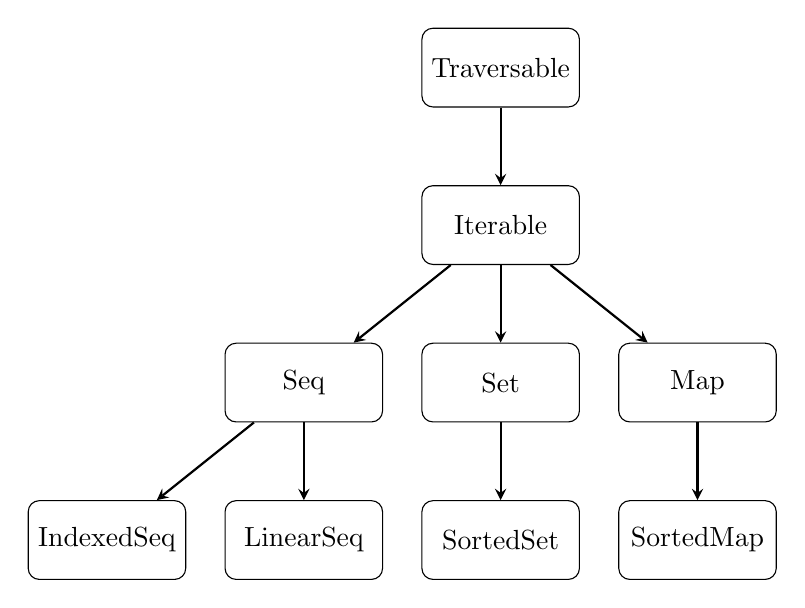
\begin{tikzpicture}[align=center, node distance=2cm]
    \node (traversable) [trait] {Traversable};
    \node (iterable) [trait, below of=traversable] {Iterable};
    \node (set) [trait, below of=iterable] {Set};
    \node (sortedset) [trait, below of=set] {SortedSet};

    \begin{scope}[node distance=25mm]
        \node (seq) [trait, left of=set] {Seq};
        \node (linearseq) [trait, left of=sortedset] {LinearSeq};
        
        \node (map) [trait, right of=set] {Map};
        \node (sortedmap) [trait, right of=sortedset] {SortedMap};
        
        \node (indexedseq) [trait, left of=linearseq] {IndexedSeq};
    \end{scope}

    \draw [arrow] (traversable) -- (iterable);

    \draw [arrow] (iterable) -- (set);
    \draw [arrow] (iterable) -- (seq);
    \draw [arrow] (iterable) -- (map);
    
    \draw [arrow] (seq) -- (indexedseq);
    \draw [arrow] (seq) -- (linearseq);
    
    \draw [arrow] (set) -- (sortedset);

    \draw [arrow] (map) -- (sortedmap);

\end{tikzpicture}
    \caption{Kokoelmien hierarkia}\label{kokoelmahierarkia}
\end{figure}


\section{Järjestykselliset kokoelmat}
\todo{Etsi parempi ilmaus järjestykselliselle}
Suorituskykyvertailuun valittiin muuttumattomista kokoelmista \code{List}, joka tyypillinen rekursiivinen linkitetty rakenne funktionaaliessa ohjelmoinnissa, ja \code{Vector}, jossa alkion haku indeksin mukaan on tehokkaampaa. Muuttuvista kokoelmista valittiin \code{Array}, joka on kiinteän kokoinen taulukko, \code{ArrayBuffer}, joka on dynaamisesti kasvava taulukko ja \code{ListBuffer}, joka on dynaamisesti kasvava linkitetty rakenne. Kaikki kyseiset muuttuvat tietorakenteet ovat tyypillisiä olio-ohjelmoinnissa käytettyjä tietorakenteita.

\code{List} on abstrakti luokka, joka kuvaa yhteen suuntaan linkitettyä rekursiivista muuttumatonta listaa, jolla on kaksi konkreettista toteutusta: \code{::} ja \code{Nil}. Epätyhjää listaa kuvaavassa luokassa \code{::} on kaksi jäsentä: alkio, jota kutsutaan listan \textit{pääksi}, ja \textit{häntä} joka kuvaa listan muita alkioita. Tyhjää listaa ja samalla listan loppumista kuvaa singleton-olio \code{Nil}. Esimerkiksi luvut 1 ja 2 sisältävä lista voidaan ilmaista näin: \code{1 :: 2 :: Nil}. Listan \code{head}-ja \code{tail}-operaatiot sekä listan alkuun lisääminen tapahtuvat vakioajassa. Aikakompleksisuus alkion hakemiselle indeksin perusteella on lineaarinen.
\cite{scalaAPI}
\cite{scalaCollections}

\code{Vector} on taulukon ominaisuuksia jäljittelevä muuttumaton tietorakenne, joka on toteutettu puurakenteena, jonka solmut ovat korkeintaan 32-alkioisia taulukoita. Lehtisolmujen taulukot sisältävät vektorin varsinaisia alkioita, ja muut solmut sisältävät alemman tason taulukoita. Jos esimerkiksi alustetaan uusi 70-alkioinen vektori, on se kolmen taulukon puu, jossa juurisolmuna olevalla taulukolla on kolme lapsitaulukkoa, joista kahdessa on 32 alkiota ja yhdessä 6 alkiota. Tämä mahdollistaa taulukoiden rakenteellisen jakamisen eri vektori-instanssien kesken, mikä vähentää kopioimista ja muistinkäyttöä. Satunnaisten haku-, muokkaus- ja poisto-operaatioiden aikakompleksisuus on log(32, N), eli operaatioiden voidaan ajatella tapahtuvan lähes vakioajassa.
\cite{scalaCollections}
\cite[Luku 4]{highPerformanceProgramming}

\code{Array} on Scalassa erityinen kokoelma, joka mahdollistaa primitiivityyppisten, viittaustyyppisten ja geneeristen alkioiden tallentamisen. Primitiivityyppisiä alkioita käsitellään ilman alkioiden käärimistä olioiksi. Esimerkiksi kokonaislukuja sisältävä \\\code{Array[Int]} kääntyy Javan \code{int[]}-taulukoksi. Kuten Javassa, taulukon koko ei voi muuttua alustamisen jälkeen. Verrattuna Javan taulukoihin \code{Array} tarjoaa kuitenkin huomattavasti enemmän operaatioita. Haku-ja muokkausoperaatiot tapahtuvat vakioajassa. Häntäoperaatio vie kuitenkin lineaarisen ajan, sillä jokainen alkio, poislukien ensimmäinen, joudutaan kopioimaan uuteen taulukkoon.
\cite{scalaCollections}

\code{ArrayBuffer} on dynaamisesti kasvava listarakenne, joka käyttää alkioiden tallentamiseen taulukkoa. Tästä johtuen useimmat operaatiot vastaavat aikakompleksisuudeltaan \code{Array}:ta. Lisäksi \code{ArrayBuffer} mahdollistaa alkion lisäämisen taulukon alkuun, loppuun sekä keskelle. Alkuun ja keskelle lisäämisen aikakompleksisuus on lineaarinen. Muut operaatiot tapahtuvat pääasiassa vakioajassa, poislukien täyteen taulukkoon lisääminen, joka vie lineaarisen ajan.
\cite{scalaCollections}

\code{ListBuffer} on dynaamisesti kasvava muuttuva kokoelma joka on toteutettu linkitettynä rakenteena. Poiketen \code{List}:stä, \code{ListBuffer} mahdollistaa alkioiden lisäämisen rakenteen alkuun ja loppuun vakioajassa. Satunnaisen alkion haku-ja muokkausoperaatiot sekä rakenteen keskelle lisääminen ovat aikakompleksisuudeltaan lineaarisia. Myös häntäoperaatio vie lineaarisen ajan, sillä kaikki hännän alkiot täytyy kopioida uuteen tietorakenteeseen.   
\cite{scalaCollections}


\section{Suorituskykyvertailut}
Tutkielmassa on käytetty kokoelmien suorituskykymittauksia kahdesta eri lähteestä: Li Haoyi:n\cite{haoyiBenchmark} ja Toby Hobsonin\cite{hobsonBenchmark} mittauksista. Haoyin mittauksissa mitataan aikaa, jonka operaatioiden suorittaminen vie, eli pienempi arvo tarkoittaa parempaa suorituskykyä. Hobsonin mittauksissa tarkastellaan operaatioiden määrää sekunnissa, jolloin suuri luku takoirttaa parempaa suorituskykyä. Hayoin mittauksissa suorituskykyä on mitattu eri kokoisilla kokoelmilla. Kaavioihin on valittu kyseisen operaation kannalta mielekkäät koot kokoelmille.

Järjestyksellisten kokoelmien tapauksessa kiinnostuksen kohteena on yleisimpien operaatioiden suorituskyky: kokoelman luominen, iterointi, alkion satunnainen haku sekä lisääminen ja häntäoperaatio. 


\subsection{Iterointi}
Iteroinnissa kokoelman jokainen alkio käydään läpi. Lähteenä käytettävissä suorituskykymittauksissa ei tutkittu rinnakkaisten kokoelmien suorituskykyä, joten iterointi tapahtui järjestyksessä. Haoyin mittauksissa \code{Array}:n iteroiminen \code{while}-silmukalla sekä \\\code{ArrayBuffer}:n iteroiminen tapahtui mittaamattoman lyhyessä tai jopa negatiivisessa ajassa, joten on kyseisiä mittauksia ei otettu huomioon. Kaaviosta \ref{iterointi_kaavio} voidaan huomata, että suorituskyvyissä ei ollut suuria eroavaisuuksia, paitsi Hobsonin mittauksissa \code{ArrayBuffer} oli 3-4 kertaa muita kokoelmia nopeampi. Haoyin mittauksissa merkittävää eroa ei ollut, vaikkakin \code{Array} oli hieman muita nopeampi.

\begin{figure}[h]
    \centering
    \definecolor{list}{HTML}{4F81BD}
\definecolor{vector}{HTML}{C0504D}
\definecolor{array}{HTML}{00FF00}
\definecolor{arraybuffer}{HTML}{9F4C7C}
\definecolor{listbuffer}{HTML}{FCBA03}

\pgfplotstableread{
    size    List    Vector  Array
    4096    14100   16200   14200
    16192   55000   62000   55600
    65536   231000  256000  228000
    262144  920000  1030000 910000
}\haoyi

\pgfplotstableread{
    collection  result
    List        396586
    Vector      321700
    Array       1226833
    ArrayBuffer 412568
    ListBuffer  3434340
}\hobson

\begin{tikzpicture}
    \begin{axis}[
        width=0.52*\textwidth,
        xshift=-2cm,
        xtick=data,
        xticklabels from table={\haoyi}{size},
        ymin=0,
        name={haoyi},
        title={Haoyi},
        xlabel={Kokoelman koko},
        legend pos=north west,
        legend style={draw=none},
    ]

    \addplot+[blue] table [y=List, x expr=\coordindex]{\haoyi};
    \addplot+[red] table [y=Vector, x expr=\coordindex]{\haoyi};
    \addplot+[green] table [y=Array, x expr=\coordindex]{\haoyi};

    \legend{List, Vector, Array, ArrayBuffer}

    \end{axis}

    \begin{axis}[
        at={(haoyi.south east)},
        xshift=1cm,
        width=0.52*\textwidth,
        ybar,
        ymin=0,
        xtick=data,
        xticklabel style={rotate=45, anchor=north east},
        title={Hobson},
        symbolic x coords={List, Vector, Array, ArrayBuffer, ListBuffer}
    ]
    
    \addplot table[x=collection, y=result]{\hobson};

\end{axis}

\end{tikzpicture}
    \caption{Iterointi}\label{iterointi_kaavio}
\end{figure}


\subsection{Satunnainen haku}
Nimensä mukaan satunnainen haku tarkoittaa alkion hakemista kokoelmasta satunnaisen indeksin perusteella. Linkitetyissä rakenteissa haku vaatii alkioiden käymistä läpi peräkkäin kunnes haettu indeksi saavutetaan. Taulukkopohjaisissa tietorakenteissa vastaavaa rajoitetta ei ole, vaan alkion muistiosoite voidaan laskea suoraan indeksin perusteella. Tämän perusteella on perusteltua olettaa taulukkojen olevan huomattavasti linkitettyjä rakenteita suorituskykyisempiä.

Hobsonin mittaukset kaaviossa \ref{satunnainenHaku_kaavio} tukevat tätä hypoteesia. \code{ListBuffer} sekä \code{List} ovat jopa useita satoja kertoja hitaampia kuin taulukoihin pohjautuvat kokoelmat. Hieman yllättäen \code{ListBuffer} on kuitenkin noin 3,5 kertaa nopeampi kuin \code{List}, vaikka \code{ListBuffer} käyttää sisäisesti alkioiden tallentamiseen \code{List}:iä. Taulukon ominaisuuksia mukaileva \code{Vector} ja \code{Array} olivat suorituskyvyltään lähes identtisiä. \code{ArrayBuffer} oli noin 15\% nopeampi kuin muut taulukkopohjaiset kokoelmat, mikä on hieman yllättävää, sillä sisäisesti alkiot tallennetaan käyttäen \code{Array}:ta.

\begin{figure}[h]
    \centering
    \pgfplotstableread{
    collection  result
    List        313253
    Vector      62082283
    Array       60777210
    ArrayBuffer 72734680
    ListBuffer  1107126
}\hobson

\begin{tikzpicture}
    \begin{axis}[
        at={(haoyi.south east)},
        ybar,
        width=12cm,
        height=9cm,
        ymin=0,
        xtick=data,
        title={Hobson},
        ylabel={ops/s},
        symbolic x coords={List, Vector, Array, ArrayBuffer, ListBuffer},
        nodes near coords,
        every node near coord/.append style={/pgf/number format/fixed},
    ]
    
    \addplot table[x=collection, y=result]{\hobson};

\end{axis}

\end{tikzpicture}
    \caption{Satunnainen haku}\label{satunnainenHaku_kaavio}
\end{figure}


\subsection{Kokoelman luominen}
Kokoelmia rakennetaan useasti lisäämällä alkioita yksi kerrallaan kokoelmaan. Joskus kokoelma luodaan toisen kokoelman tai kokoelmatyypin alkioista. Taulukkoa (\code{Array}) luotaessa täytyy yleensä päättää miten monen alkion taulukko luodaan. Mikäli täyteen taulukkoon halutaan lisätä alkioita, täytyy luoda uusi suurempi taulukko ja kopioida kaikki alkiot alkuperäisestä taulukosta uuteen taulukkoon ja lisätä uusi alkio uuteen taulukkoon. Taulukon kaikkien alkioiden kopiointi uuteen taulukkoon todennäköisesti huonontaa suorituskykyä huomattavasti.

Hayoin vertailuissa (kaavio \ref{kokoelmanLuominen_kaavio}) on testattu useita tapoja kokoelmien luomiseen. \code{Array:+} kuvastaa tilannetta, jossa luodaan kokoelma lisäämällä alkio täyteen taulukkoon. Oletetusti sen suorituskyky on koko vertailun huonoin. \code{Array}-prealloc kuvaa tilannetta, jossa luodaan valmiiksi oikean kokoinen taulukko, ja sen suorituskyky on vertailun paras.

\code{List::} rakentaa linkitetyn rakenteen lisäämällä alkioita linkitetyn listan alkuun, ja sen on ilmoitettu tapahtuvan vakioajassa. \cite{scalaCollections} Hayoin mittaukset osoittavat tämän todeksi ja ainoastaan \code{Array}-prealloc oli \code{List}:aa suorituskykyisempi.

Kun \code{ArrayBuffer}:n sisäinen taulukko tulee täyteen, luodaan uusi, kaksi kertaa alkuperäistä suurempi, taulukko ja vanhan taulukon arvot kopioidaan uuteen. Suorituskyky on linkitettyä rakennetta huonompi, mutta hieman \code{Array.toVector}:ia parempi.

\code{Vector:+} aikakompleksisuuden pitäisi olla lähes vakio \cite{scalaCollections}, mutta mittausten perusteella suorituskyky on varsin heikko. Erityisesti kun luodaan yli 1024 alkion kokoelmia ja sisäiseen puurakenteeseen tulee yksi taso lisää, suorituskyky heikkenee merkittävästi. Suorituskykyisempi tapa luoda \code{Vector} on luoda toinen kokoelma ja kutsua sen \code{toVector}-metodia. Haoyin mittausten \code{Array.toVector} on tilanne, jossa luodaan \code{Array} pre-alloc-tyylisesti ja luodaan sen pohjalta \code{Vector}. Suorituskyky on huomattavasti parempi kuin lisäämällä alkioita yksi kerrallaan.

\begin{figure}[h]
    \centering
    \pgfplotstableread{
    size    List::  Vector:+ Array.toVector Array:+ Array-prealloc  ArrayBuffer
    64      301     1730     903            1460    186             691
    1024    4900    28600    12850          260000  2710            10840
    4096    19800   324000   51100          3170000 11000           43000
}\haoyi

\begin{tikzpicture}
    \begin{axis}[
        width=12cm,
        height=9cm,
        xtick=data,
        xticklabels from table={\haoyi}{size},
        ymin=0,
        ymax=55000,
        name={haoyi},
        title={Haoyi},
        ylabel={ns},
        xlabel={Kokoelman koko},
        legend pos=north west,
        legend style={draw=none},
    ]

    \addplot+[blue] table [y=List::, x expr=\coordindex]{\haoyi};
    \addplot+[red] table [y=Vector:+, x expr=\coordindex]{\haoyi};
    \addplot+[violet] table [y=Array.toVector, x expr=\coordindex]{\haoyi};
    \addplot+[green] table [y=Array:+, x expr=\coordindex]{\haoyi};
    \addplot+[black] table [y=Array-prealloc, x expr=\coordindex]{\haoyi};
    \addplot+[brown] table [y=ArrayBuffer, x expr=\coordindex]{\haoyi};

    \legend{List::, Vector:+, Array.toVector, Array:+, Array-prealloc, ArrayBuffer}

    \end{axis}

\end{tikzpicture}
    \caption{Kokoelman luominen}\label{kokoelmanLuominen_kaavio}
\end{figure}


\begin{figure}[h]
    \centering
    \definecolor{list}{HTML}{4F81BD}
\definecolor{vector}{HTML}{C0504D}
\definecolor{array}{HTML}{00FF00}
\definecolor{arraybuffer}{HTML}{9F4C7C}
\definecolor{listbuffer}{HTML}{FCBA03}

\pgfplotstableread{
    collection              result
    List                    307
    List(prepend)           39799
    Vector                  26882
    Array*                  49790
    ArrayBuffer             173677
    ListBuffer              69692
    ListBuffer(prepend)     39799
}\hobson

% "As you can see in the source, I actually allocated a 1000 element array then copied each element into the slot so it’s not strictly an append operation."

\begin{tikzpicture}
    \begin{axis}[
        at={(haoyi.south east)},
        ybar,
        width=12cm,
        height=9cm,
        ymin=0,
        xtick=data,
        title={Hobson},
        symbolic x coords={List, List(prepend), Vector, Array*, ArrayBuffer, ListBuffer, ListBuffer(prepend)},
        xticklabel style={rotate=45, anchor=north east},
    ]
    
    \addplot table[x=collection, y=result]{\hobson};

\end{axis}

\end{tikzpicture}
    \caption{Kokoelman loppuun lisääminen}\label{kokoelmanLoppuunLisaaminen_kaavio}
\end{figure}

\subsection{Kokoelman loppuun lisääminen}
Asetelma Hobsonin mittauksessa kokoelman loppuun lisäämisestä on hieman samankaltainen kuin Haoyin kokoelman luomisen mittauksessa, mutta varsinkin \code{List} suoriutuu loppuun lisäämisestä huomattavasti heikommin. Loppuun lisättäessä, täytyy jokainen alkio kopioida uuteen kokoelmaan ja uusi alkio lisätä uuden kokoelman loppuun. \code{List}-prepend tarkoittaa tilannetta jossa alkio lisätään rakenteen alkuun, ja kokoelman järjestys käännetään. Kaaviosta \ref{kokoelmanLoppuunLisaaminen_kaavio} voidaan huomata, että tällä tavoin suorituskyky on jopa yli 100 kertaa parempi.

Muuttuvasta linkitetystä rakenteesta, \code{ListBuffer}:sta on mittaus kummallakin edellisessä kappaleessa mainitulla tavalla. Suoraan kokoelman loppuun lisäämisellä saavutetaan paras suorituskyky, ja se on jopa yli 70\% parempi kuin lisäämällä alkuun ja kääntämällä kokoelman järjestys. Prepend-tyylillä suorituskyky on identtinen \code{List}-prepend kanssa. 

Taulukoista \code{ArrayBuffer} suoriutuu selvästi parhaiten, ollen yli kolme kertaa parempi kuin seuraavaksi paras taulukkorakenne \code{Array}. On syytä huomioida, että kyseisessä mittauksessa luodaan valmiiksi oikean kokoinen \code{Array}. \code{Vector} suoriutuu tästäkin mittauksesta yllättävän huonosti, ollen noin 50\% huonompi kuin \code{Array} ja 30\% huonompi kuin \code{List}-prepend.


\subsection{Häntäoperaatio}

\begin{figure}[h]
    \centering
    \pgfplotstableread{
    size    List    Vector  Array   ArrayBuffer
    16      21      425     582     43
    64      100     1970    4517    166
    256     420     11800   55500   630
    1024    2100    58400   82100   2510
}\haoyi

\begin{tikzpicture}
    \begin{axis}[
        width=12cm,
        height=9cm,
        xtick=data,
        xticklabels from table={\haoyi}{size},
        ymin=0,
        ymax=4000,
        title={Haoyi},
        ylabel={ns},
        xlabel={Kokoelman koko},
        legend pos=north east,
        legend style={draw=none},
    ]

    \addplot+[blue] table [y=List, x expr=\coordindex]{\haoyi};
    \addplot+[red] table [y=Vector, x expr=\coordindex]{\haoyi};
    \addplot+[green] table [y=Array, x expr=\coordindex]{\haoyi};
    \addplot+[violet] table [y=ArrayBuffer, x expr=\coordindex]{\haoyi};

    \legend{List, Vector, Array, ArrayBuffer}
\end{axis}
\end{tikzpicture}
    \caption{Häntäoperaatio}\label{hantaoperaatio_kaavio}
\end{figure}

Haoyin häntäoperaation suorituskykyä mittaavassa tutkimuksessa aloitetaan n-kokoisesta kokoelmasta ja tehdään häntäoperaatiota jäljelle jäävälle kokoelmalle, kunnes jäljellä on tyhjä kokoelma. Mittauksen tulos on kulunut aika, jolloin pieni arvo tarkoittaa hyvää suorituskykyä. Kaaviossa \ref{hantaoperaatio_kaavio} on mittauksen tulokset.

\code{List} suoriutuu oletetusti parhaiten. Muuttumattoman linkitetyn rakenteen häntään saadaan viittaus yksinkertaisesti palauttamalla ensimmäisen alkion seuraaja, ja se tapahtuu aina vakioajassa. \code{ArrayBuffer} suoriutui mittauksessa vain hieman \code{List}:iä huonommin. 

Selvästi huonoiten suoriutui \code{Array}. Tulos on oletettu, sillä jokaisella häntäoperaatiolla kaikki paitsi taulukon ensimmäinen alkio täytyy kopioida uuteen taulukkoon. \code{Vector} on hieman \code{Array}:ta parempi, mutta sen suorituskyky on 256:n alkion kokoelmalla jo noin 20 kertaa huonompi kuin kahdella suorituskykyisimmällä kokoelmalla.
